% !TEX root = ../discretemath.tex

\section{Матричные игры (с нулевой суммой) и примеры}

\subsection{Постановка задачи}

Игра двух игроков с нулевой суммой задаётся \emph{матрицей выигрышей}
\[
A=\begin{pmatrix} a_{11} & \cdots & a_{1n} \\ \vdots & & \vdots \\ a_{m1} & \cdots & a_{mn}\end{pmatrix}\in\mathbb{R}^{m\times n}.
\]
Правила: 1-й игрок независимо выбирает строку $i$, 2-й — столбец $j$, после чего 2-й платит 1-му сумму $a_{ij}$. Значит, 1-й игрок \emph{максимизирует} выигрыш, 2-й — \emph{минимизирует}.

\subsection{Чистые стратегии: цена игры и седловая точка}

\begin{Definition}{Нижняя и верхняя цены игры}{}
	\emph{Нижняя цена} (что гарантирует себе 1-й игрок):
	\[
	\alpha=\max_i\min_j a_{ij}.
	\]
	\emph{Верхняя цена} (что гарантирует себе 2-й игрок):
	\[
	\beta=\min_j\max_i a_{ij}.
	\]
\end{Definition}

Выбирая строку $i^*=\arg\max_i\min_j a_{ij}$, 1-й игрок обеспечивает выигрыш не менее $\alpha$ при любом ответе соперника; выбирая $j^*=\arg\min_j\max_i a_{ij}$, 2-й игрок ограничивает свои потери величиной $\beta$.

\begin{Theorem}{Всегда $\alpha\le\beta$}{}
	Для любой матрицы $A\in\mathbb{R}^{m\times n}$ выполнено $\alpha\le\beta$.
\end{Theorem}

\begin{proof}
	Для любых $i,j$ имеем $\min_{j'}a_{ij'}\le a_{ij}\le\max_{i'}a_{i'j}$. Беря $\max_i$ слева и $\min_j$ справа:
	\[
	\alpha=\max_i\min_{j'}a_{ij'}\le\min_j\max_{i'}a_{i'j}=\beta.
	\]
\end{proof}

\begin{Definition}{Седловая точка}{}
	Если $\alpha=\beta$, то у игры есть \emph{цена} $\upsilon=\alpha=\beta$ и \emph{седловая точка} $(i^*,j^*)$:
	\[
	a_{ij^*}\le a_{i^*j^*}\le a_{i^*j}\quad\text{для всех }i,j.
	\]
	То есть $a_{i^*j^*}$ — одновременно минимум в своей строке и максимум в своём столбце.
\end{Definition}

\begin{Remark}{}{}
	Замена $A$ на $-A^{\top}$ меняет роли игроков местами.
\end{Remark}

\begin{Statement}{Единственность значения в сёдлах}{}
	Если у $A$ есть два седла $(i_1,j_1)$ и $(i_2,j_2)$, то все четыре элемента $a_{i_1j_1},a_{i_1j_2},a_{i_2j_1},a_{i_2j_2}$ равны $\upsilon$.
\end{Statement}

\begin{proof}
	Из седла в $(i_1,j_1)$: $a_{i_2j_1}\le a_{i_1j_1}\le a_{i_1j_2}$. Из седла в $(i_2,j_2)$: $a_{i_1j_2}\le a_{i_2j_2}\le a_{i_2j_1}$. Тогда
	\[
	a_{i_1j_1}\le a_{i_1j_2}\le a_{i_2j_2}\le a_{i_2j_1}\le a_{i_1j_1},
	\]
	поэтому все четыре значения совпадают.
\end{proof}

\begin{Example}{Матрица $3\times3$ с седловой точкой}{}
	\[
	A=\begin{pmatrix} 2 & 4 & 7 \\ 6 & \mathbf{5} & 6 \\ 3 & 4 & 1 \end{pmatrix}.
	\]
	Минимумы по строкам $2,5,1$, поэтому $\alpha=\max(2,5,1)=5$. Максимумы по столбцам $6,5,7$, поэтому $\beta=\min(6,5,7)=5$. Так как $\alpha=\beta=5$, цена игры $5$, седло — элемент $a_{22}=5$.
\end{Example}

\begin{figure}[H]
	\centering
	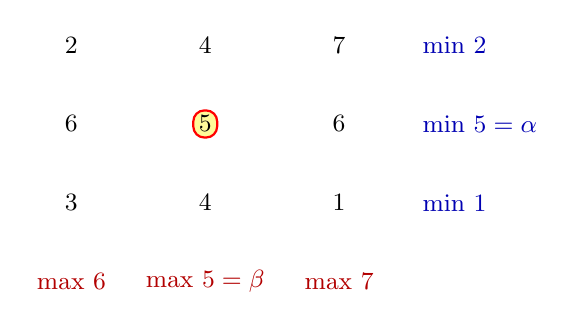
\begin{tikzpicture}[font=\small, x=1.7cm, y=1.0cm]
		% элементы
		\foreach \x/\y/\val in {0/0/2, 1/0/4, 2/0/7,
			0/-1/6, 2/-1/6, 0/-2/3, 1/-2/4, 2/-2/1}{
			\node at (\x,\y) {$\val$};
		}
		% седло
		\node[draw=red, thick, fill=yellow!40, rounded corners, inner sep=2pt] at (1,-1) {$5$};
		% минимумы по строкам
		\node[blue!70!black, anchor=west] at (2.55,0) {min $2$};
		\node[blue!70!black, anchor=west] at (2.55,-1) {min $5=\alpha$};
		\node[blue!70!black, anchor=west] at (2.55,-2) {min $1$};
		% максимумы по столбцам
		\node[red!70!black] at (0,-3) {max $6$};
		\node[red!70!black] at (1,-3) {max $5=\beta$};
		\node[red!70!black] at (2,-3) {max $7$};
	\end{tikzpicture}
	\caption{Седловая точка матрицы $3\times3$. Элемент $a_{22}=5$ — минимум в своей строке (синие) и максимум в своём столбце (красные). Совпадение $\alpha=\beta=5$ даёт цену игры в чистых стратегиях.}
\end{figure}

\subsection{Смешанные стратегии}

При чистых стратегиях гарантируется лишь $\alpha\le\upsilon\le\beta$. Чтобы всегда достигать точной цены, вводят \emph{смешанные} (рандомизированные) стратегии.

\begin{Definition}{Смешанные стратегии и ожидаемый выигрыш}{}
	Смешанная стратегия 1-го игрока — вектор $\vec p=(p_1,\dots,p_m)$, $p_i\ge 0$, $\sum p_i=1$; 2-го — $\vec q=(q_1,\dots,q_n)$, $q_j\ge 0$, $\sum q_j=1$. Ожидаемый выигрыш 1-го игрока:
	\[
	E(\vec p,\vec q)=\sum_{i=1}^m\sum_{j=1}^n a_{ij}\,p_i\,q_j.
	\]
\end{Definition}

\begin{Definition}{Оптимальная пара стратегий}{}
	Пара $(\vec p^{\,*},\vec q^{\,*})$ \emph{оптимальна} (равновесие в смешанных стратегиях), если для всех $\vec p,\vec q$:
	\[
	E(\vec p,\vec q^{\,*})\le E(\vec p^{\,*},\vec q^{\,*})\le E(\vec p^{\,*},\vec q).
	\]
	Число $\upsilon=E(\vec p^{\,*},\vec q^{\,*})$ — \emph{цена игры}.
\end{Definition}

\begin{Statement}{Выпуклость множества оптимумов}{}
	Пусть $(\vec p^{\,*},\vec q^{\,*})$ и $(\vec p^{\,\prime},\vec q^{\,\prime})$ — две оптимальные пары. Тогда:
	\begin{enumerate}
		\item $E(\vec p^{\,*},\vec q^{\,*})=E(\vec p^{\,\prime},\vec q^{\,\prime})=\upsilon$;
		\item для любых $\alpha,\beta\in[0,1]$ пара $\bigl(\alpha\vec p^{\,*}+(1-\alpha)\vec p^{\,\prime},\ \beta\vec q^{\,*}+(1-\beta)\vec q^{\,\prime}\bigr)$ тоже оптимальна.
	\end{enumerate}
\end{Statement}

\begin{proof}
	\textbf{(1)} Из оптимальности $(\vec p^{\,*},\vec q^{\,*})$: $E(\vec p^{\,*},\vec q^{\,*})\le E(\vec p^{\,*},\vec q^{\,\prime})\le E(\vec p^{\,\prime},\vec q^{\,\prime})$; симметрично в обратную сторону, откуда равенство значений $=\upsilon$.

	\textbf{(2)} По линейности $E$ по каждому аргументу: для любого $\vec q$
	\[
	E\!\bigl(\vec p,\ \beta\vec q^{\,*}+(1-\beta)\vec q^{\,\prime}\bigr)
	=\beta E(\vec p,\vec q^{\,*})+(1-\beta)E(\vec p,\vec q^{\,\prime})\le\upsilon,
	\]
	\[
	E\!\bigl(\alpha\vec p^{\,*}+(1-\alpha)\vec p^{\,\prime},\ \vec q\bigr)
	=\alpha E(\vec p^{\,*},\vec q)+(1-\alpha)E(\vec p^{\,\prime},\vec q)\ge\upsilon.
	\]
	Значит, выпуклая комбинация удовлетворяет определению оптимальной пары.
\end{proof}

\begin{Example}{Матрица $2\times2$}{}
	\[
	A=\begin{pmatrix} -1 & 3 \\ 3 & -5\end{pmatrix},\qquad
	\vec p=(p,1-p),\ \vec q=(q,1-q).
	\]
	Ожидаемый выигрыш:
	\[
	E(p,q)=-pq+3p(1-q)+3(1-p)q-5(1-p)(1-q)=-5+8p+8q-12pq.
	\]
	При фиксированном $p$: $E(p,q)=(-5+8p)+(8-12p)q$. Если $p^*\ne\tfrac23$, коэффициент при $q$ ненулевой, и минимум по $q$ достигается в чистой стратегии $q^*\in\{0,1\}$; но тогда и оптимальный ответ 1-го игрока чист ($p^*\in\{0,1\}$), что противоречиво. Значит, $p^*=\tfrac23$, и аналогично $q^*=\tfrac23$. Проверка:
	\[
	E\!\left(p,\tfrac23\right)=\tfrac13\ \forall p,\qquad E\!\left(\tfrac23,q\right)=\tfrac13\ \forall q.
	\]
	Итого $\vec p^{\,*}=\vec q^{\,*}=\left(\tfrac23,\tfrac13\right)$, цена $\upsilon=\tfrac13$.
\end{Example}
